\documentclass[tikz,border=0pt]{standalone}
\usepackage[utf8]{inputenc}
\usepackage[T1]{fontenc}
\usepackage{lmodern}
\usepackage{amsmath,amssymb}
\usetikzlibrary{arrows.meta,positioning,fit,calc,backgrounds,shapes.geometric,decorations.pathreplacing}
\definecolor{navy}{HTML}{163A5F}
\definecolor{blue}{HTML}{2C6EAF}
\definecolor{lightblue}{HTML}{EAF2F8}
\definecolor{midblue}{HTML}{CFE1F2}
\definecolor{graytext}{HTML}{4A5560}
\definecolor{lightgray}{HTML}{F4F6F8}
\definecolor{green}{HTML}{3C8D73}
\definecolor{lightgreen}{HTML}{E8F5EF}
\definecolor{red}{HTML}{B24A4A}
\definecolor{lightred}{HTML}{FBEDEE}
\tikzset{
  title/.style={font=\sffamily\bfseries\fontsize{16}{18}\selectfont,text=navy,anchor=west},
  subtitle/.style={font=\sffamily\bfseries\fontsize{11}{13}\selectfont,text=navy},
  body/.style={font=\sffamily\fontsize{9.2}{11}\selectfont,text=graytext,align=left},
  small/.style={font=\sffamily\fontsize{8}{9.4}\selectfont,text=graytext,align=left},
  tinylabel/.style={font=\sffamily\fontsize{7.2}{8.4}\selectfont,text=graytext},
  panel/.style={rounded corners=3pt,draw=midblue,fill=white,line width=0.6pt},
  box/.style={rounded corners=2pt,draw=midblue,fill=lightblue,line width=0.6pt},
  worker/.style={rounded corners=2pt,draw=blue,dashed,line width=0.7pt,fill=white},
  task/.style={rounded corners=2pt,draw=blue,fill=lightblue,minimum width=0.85cm,minimum height=0.55cm,font=\sffamily\bfseries\small,text=navy},
  file/.style={draw=blue,fill=white,minimum width=0.55cm,minimum height=0.42cm,font=\sffamily\small,text=navy},
  arr/.style={-{Stealth[length=2.4mm,width=1.8mm]},draw=blue,line width=0.9pt},
  arrthin/.style={-{Stealth[length=2mm,width=1.5mm]},draw=blue,line width=0.7pt},
  arrred/.style={-{Stealth[length=2mm,width=1.5mm]},draw=red,dashed,line width=0.8pt},
  arrgreen/.style={-{Stealth[length=2mm,width=1.5mm]},draw=green,dotted,line width=1pt}
}
\begin{document}

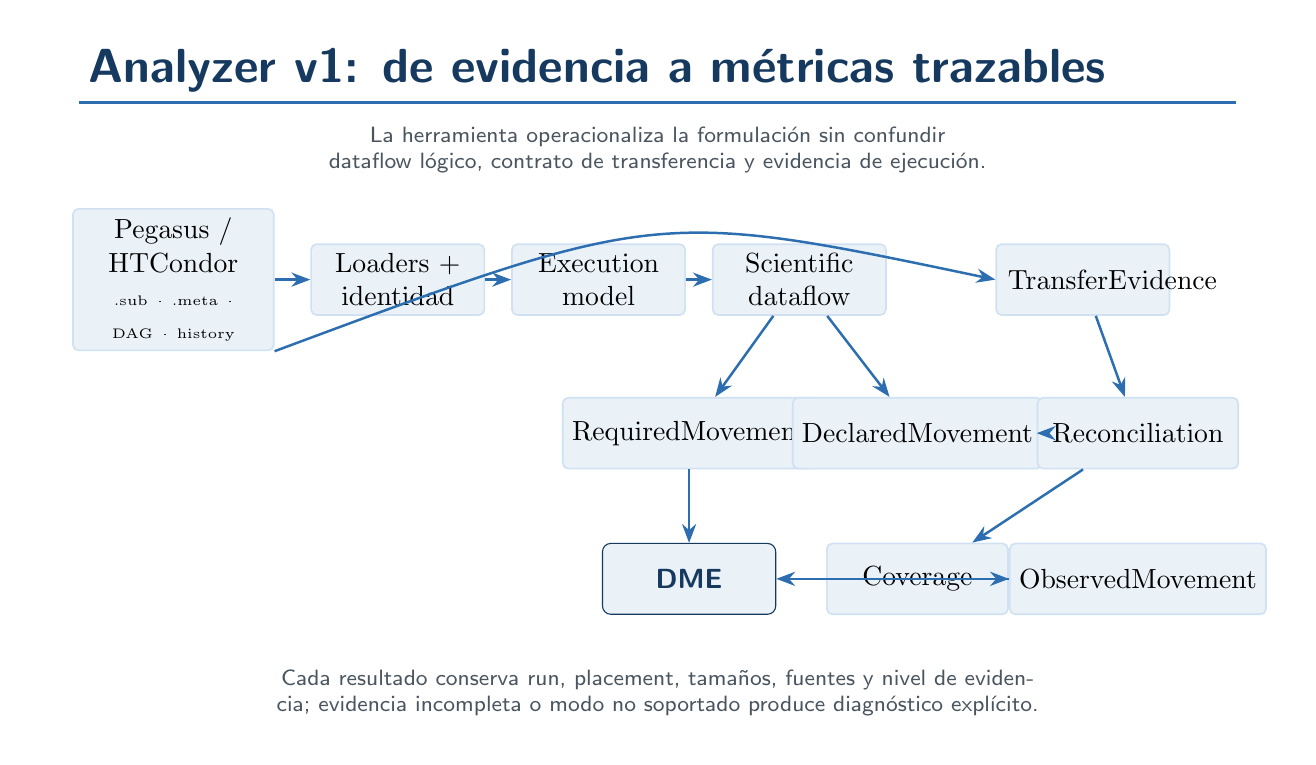
\begin{tikzpicture}[x=1cm,y=1cm]
\path[use as bounding box] (0,0) rectangle (16,9);
\node[title] at (0.65,8.45) {Analyzer v1: de evidencia a métricas trazables};
\draw[blue,line width=1pt] (0.65,8.05)--(15.35,8.05);
\node[small,text width=14cm,align=center] at (8,7.45) {La herramienta operacionaliza la formulación sin confundir dataflow lógico, contrato de transferencia y evidencia de ejecución.};

\node[box,minimum width=2.55cm,minimum height=0.9cm,text width=2.2cm,align=center] (src) at (1.85,5.8) {Pegasus / HTCondor\\\tiny .sub · .meta · DAG · history};
\node[box,minimum width=2.2cm,minimum height=0.9cm,text width=1.9cm,align=center] (load) at (4.7,5.8) {Loaders + identidad};
\node[box,minimum width=2.2cm,minimum height=0.9cm,text width=1.9cm,align=center] (em) at (7.25,5.8) {Execution model};
\node[box,minimum width=2.2cm,minimum height=0.9cm,text width=1.9cm,align=center] (df) at (9.8,5.8) {Scientific dataflow};
\node[box,minimum width=2.2cm,minimum height=0.9cm,text width=1.9cm,align=center] (ev) at (13.4,5.8) {TransferEvidence};
\draw[arr] (src)--(load); \draw[arr] (load)--(em); \draw[arr] (em)--(df); \draw[arr] (src.south east).. controls (8.0,6.7) ..(ev.west);

\node[box,minimum width=2.55cm,minimum height=0.9cm] (req) at (8.4,3.85) {RequiredMovement};
\node[box,minimum width=2.55cm,minimum height=0.9cm] (decl) at (11.3,3.85) {DeclaredMovement};
\node[box,minimum width=2.55cm,minimum height=0.9cm] (rec) at (14.1,3.85) {Reconciliation};
\draw[arr] (df)--(req); \draw[arr] (df)--(decl); \draw[arr] (decl)--(rec); \draw[arr] (ev)--(rec);

\node[box,minimum width=2.3cm,minimum height=0.9cm] (cov) at (11.3,2.0) {Coverage};
\node[box,minimum width=2.55cm,minimum height=0.9cm] (obs) at (14.1,2.0) {ObservedMovement};
\node[rounded corners=3pt,draw=navy,fill=lightblue,minimum width=2.2cm,minimum height=0.9cm,font=\sffamily\bfseries,text=navy] (dme) at (8.4,2.0) {DME};
\draw[arr] (rec)--(cov); \draw[arr] (cov)--(obs); \draw[arr] (req)--(dme); \draw[arr] (obs)--(dme);
\node[small,text width=14cm,align=center] at (8,0.55) {Cada resultado conserva run, placement, tamaños, fuentes y nivel de evidencia; evidencia incompleta o modo no soportado produce diagnóstico explícito.};
\end{tikzpicture}
\end{document}
